\chapter{Programming}\label{chap:programming}
This project required over $450$ labelings of various forests, all of which were found by hand. At around $200$ labelings it became clear that due to the sheer number of labelings being done, just probablistically some labelings would (1) have typos (2) have incorrect computations and (3) violate some constraint of the labeling.

All this programming began because we wanted some sort of local program that could display the labelings, so we could check with some level of certainty that they were isomorphic to the forest being worked with. Everything we found displayed graphs but didn't allow for dragging nodes and/or interacting with graphs at a high level. So we decided to make our own programs.

There are $3$ groups of programs in a dedicated github repository that we provide links for, for the sake of space. Note: the requirements to run these are:

\setlist[enumerate,1]{label=(\arabic*)}
\begin{enumerate}
  \item A Python 3.13 installation
  \item The NetworkX python library
  \item the pygame or pygame-ce python library
  \item the itertools python library
  \item the z3 python library
\end{enumerate}
It should be clear when looking at the code what the dependencies are. If you use pip in vscode, you may simply input: 
\begin{verbatim}
py -m pip install #enter library name here
# OR
python -m pip install #enter library name here
\end{verbatim}
depending on how you installed python installing packages may not work this way. Anaconda is a popular python IDE/installation that comes with some of these most likely.

\section{Tikzgrapher}

This is an earlier version of a program named \textit{tikzgrapher} that was specifically build with displaying (1-2-3)-labelings and 1-rotational (1-2-3)-labelings. There is a less restrictive version where arguments are optional and customizable (custom edge and vertex labelings, colorings of vertices, no side tab for squares containing lengths). Here is a link to this project: \url{https://github.com/tucxy/Thesis-Programs/blob/main/graph_visualization.py}

These are the features added, ordered earliest to latest to this older build of tikzgrapher:\newline
\setlist[enumerate,1]{label=(\arabic*)}
\begin{enumerate}
  \item Outputs a list of NetworkX graphs together on one page, starting from top to bottom.
  \item Reduces vertices modulo $n$ and computes the standard edge length for each edge modulo $n$, and has the subscript as the additive edge length $\ell{7}^{+}$.
  \item Uses longest path search algorithm and by default displays the longest path of graph in the center row of a grid of coordinates, then displays nodes coming off of that row.
  \item Has a tab on the left that displays all standard edge lengths $\ell$ and a chart for the subscript labels of the labelings in order. The window with the tab open looks similar to Figure \ref{fig:K21labelingex} except it doesn't have colored edges.
  \item Allows user to save displayed graphs as a tikz graph in a standalone \LaTeX file to a specified path
\end{enumerate}
We have every single forest labeling in notebooks that import tikzgrapher. If you simply uncomment below a forest, a pygame will pop out and display the labeling. Here are links to those notebooks:
\begin{enumerate}
  \item $\sigma^{+-}$-labelings: \url{https://github.com/tucxy/Thesis-Programs/blob/main/sigma.py}
  \item (1-2-3)-labelings: \url{https://github.com/tucxy/Thesis-Programs/blob/main/7mod14.py}
  \item 1-rotational (1-2-3)-labelings: \url{https://github.com/tucxy/Thesis-Programs/blob/main/8mod14.py}
  \item $\mathbf{T_{7}^{11}\sqcup T_{2}^{1}}$-decomposition of $K_{21}$ and $K_{22}$: \url{https://github.com/tucxy/Thesis-Programs/blob/main/starpath.py}
\end{enumerate}


\begin{figure}[H]
  \centering
  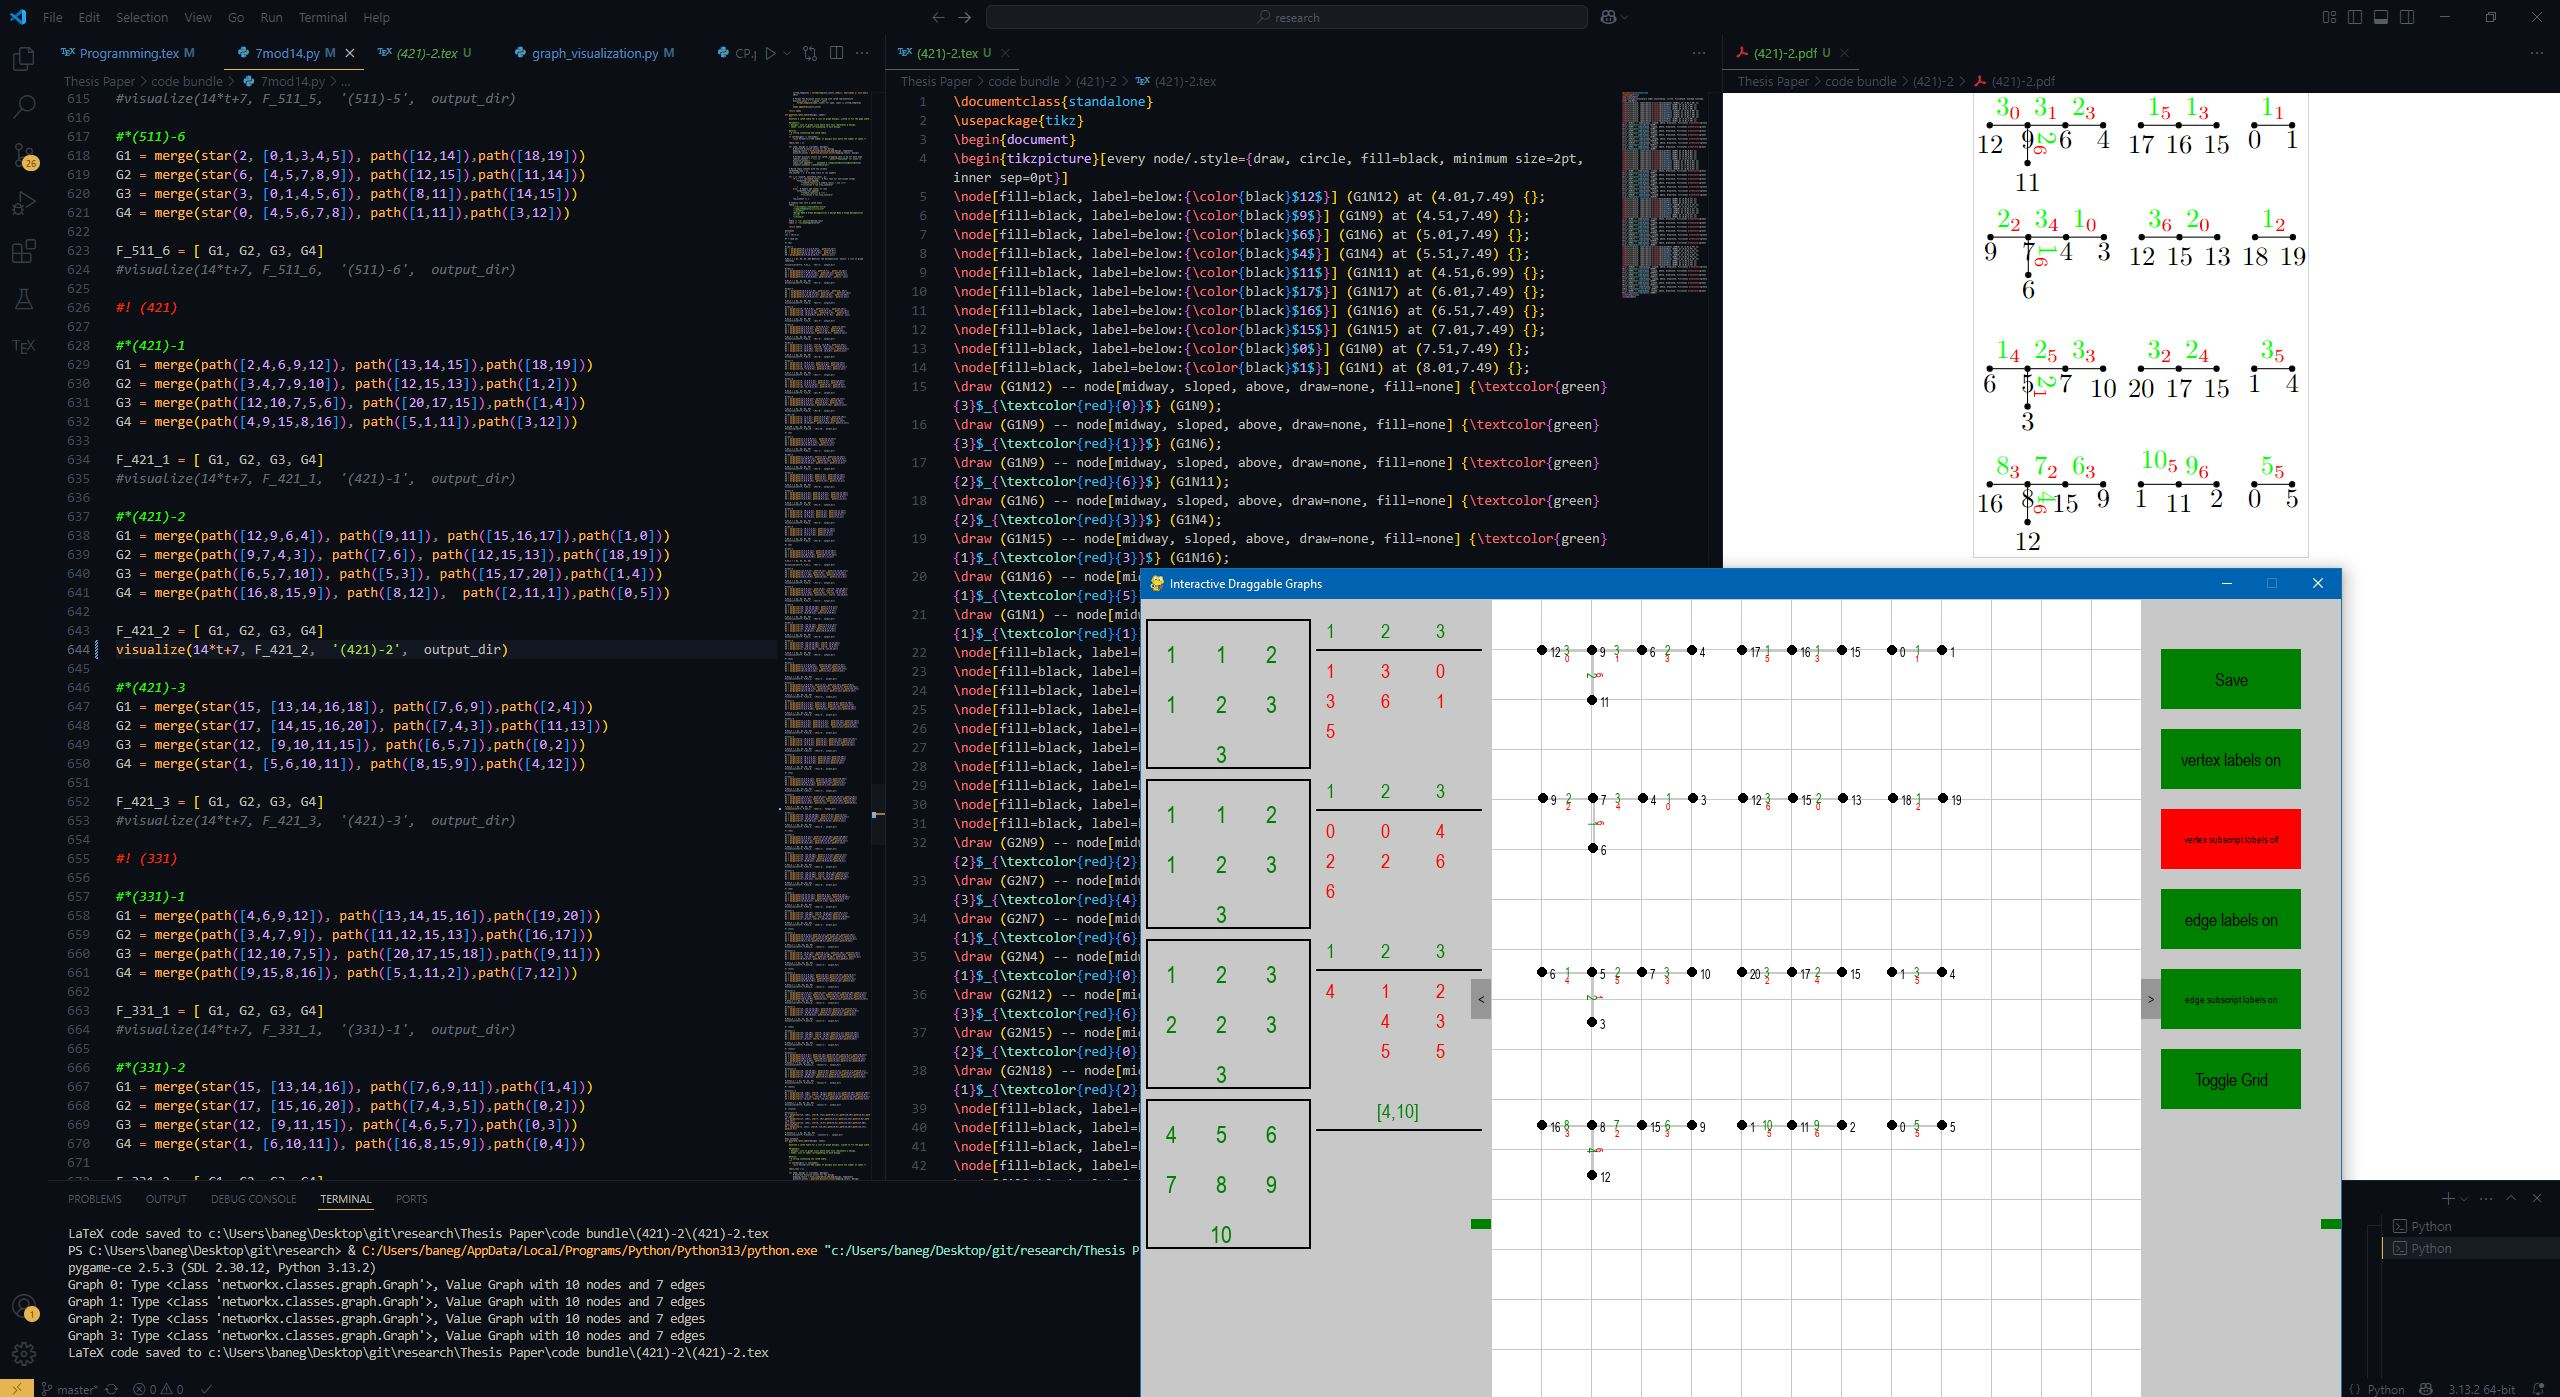
\includegraphics[width=\textwidth]{standalone/Images/snippet_long.JPG}
  \caption{A snippet of \textit{tikzgrapher}}
  \label{fig:TGsnippet}
\end{figure}


Once again, this version is no longer being updated, the following link will take you to the latest version: \url{https://github.com/tucxy/Programming/tree/main/Python/tikzgrapher} \newline

\section{Labeling Solvers}
This next program is a bit more ambitious. After all labelings were found (of course) we thought, "Hey what if we didn't have to find these by hand?" Initially, we tried to use a genetic learning algorithm but found that the fitness function was too rigid, and realized that reinforcement learning was not the way to go. We found much more success using constraint programming. Using the \text{z3} SAT solver, we created (1) a solver that outputs a $\sigma^{+-}$-labeling of a graph (if it exists) (2) a graceful labeling of a graph (3) a solver that oututs a more generalized version of the (1-2-3)-labeling for a graph on $m$ edges in $K_{2mt+r}$ where $r$ is idempotent modulo $2m$.



The $\sigma^{+-}$-labeling is quite fast, but the other labelings can take up to five minutes or so. I the future, we hope to translate this code to C++, to hopefully speed up the process. As of now, it does work however, but the beefier the processor, the better since it is in Python. Here are the links to this project:

\begin{enumerate}
  \item  Labeling Solvers: \url{https://github.com/tucxy/Thesis-Programs/blob/main/CP.py}
  \item  Notebook to test the solvers: \url{https://github.com/tucxy/Thesis-Programs/blob/main/main.py}
\end{enumerate}

\begin{figure}[H]
  \begin{center}
  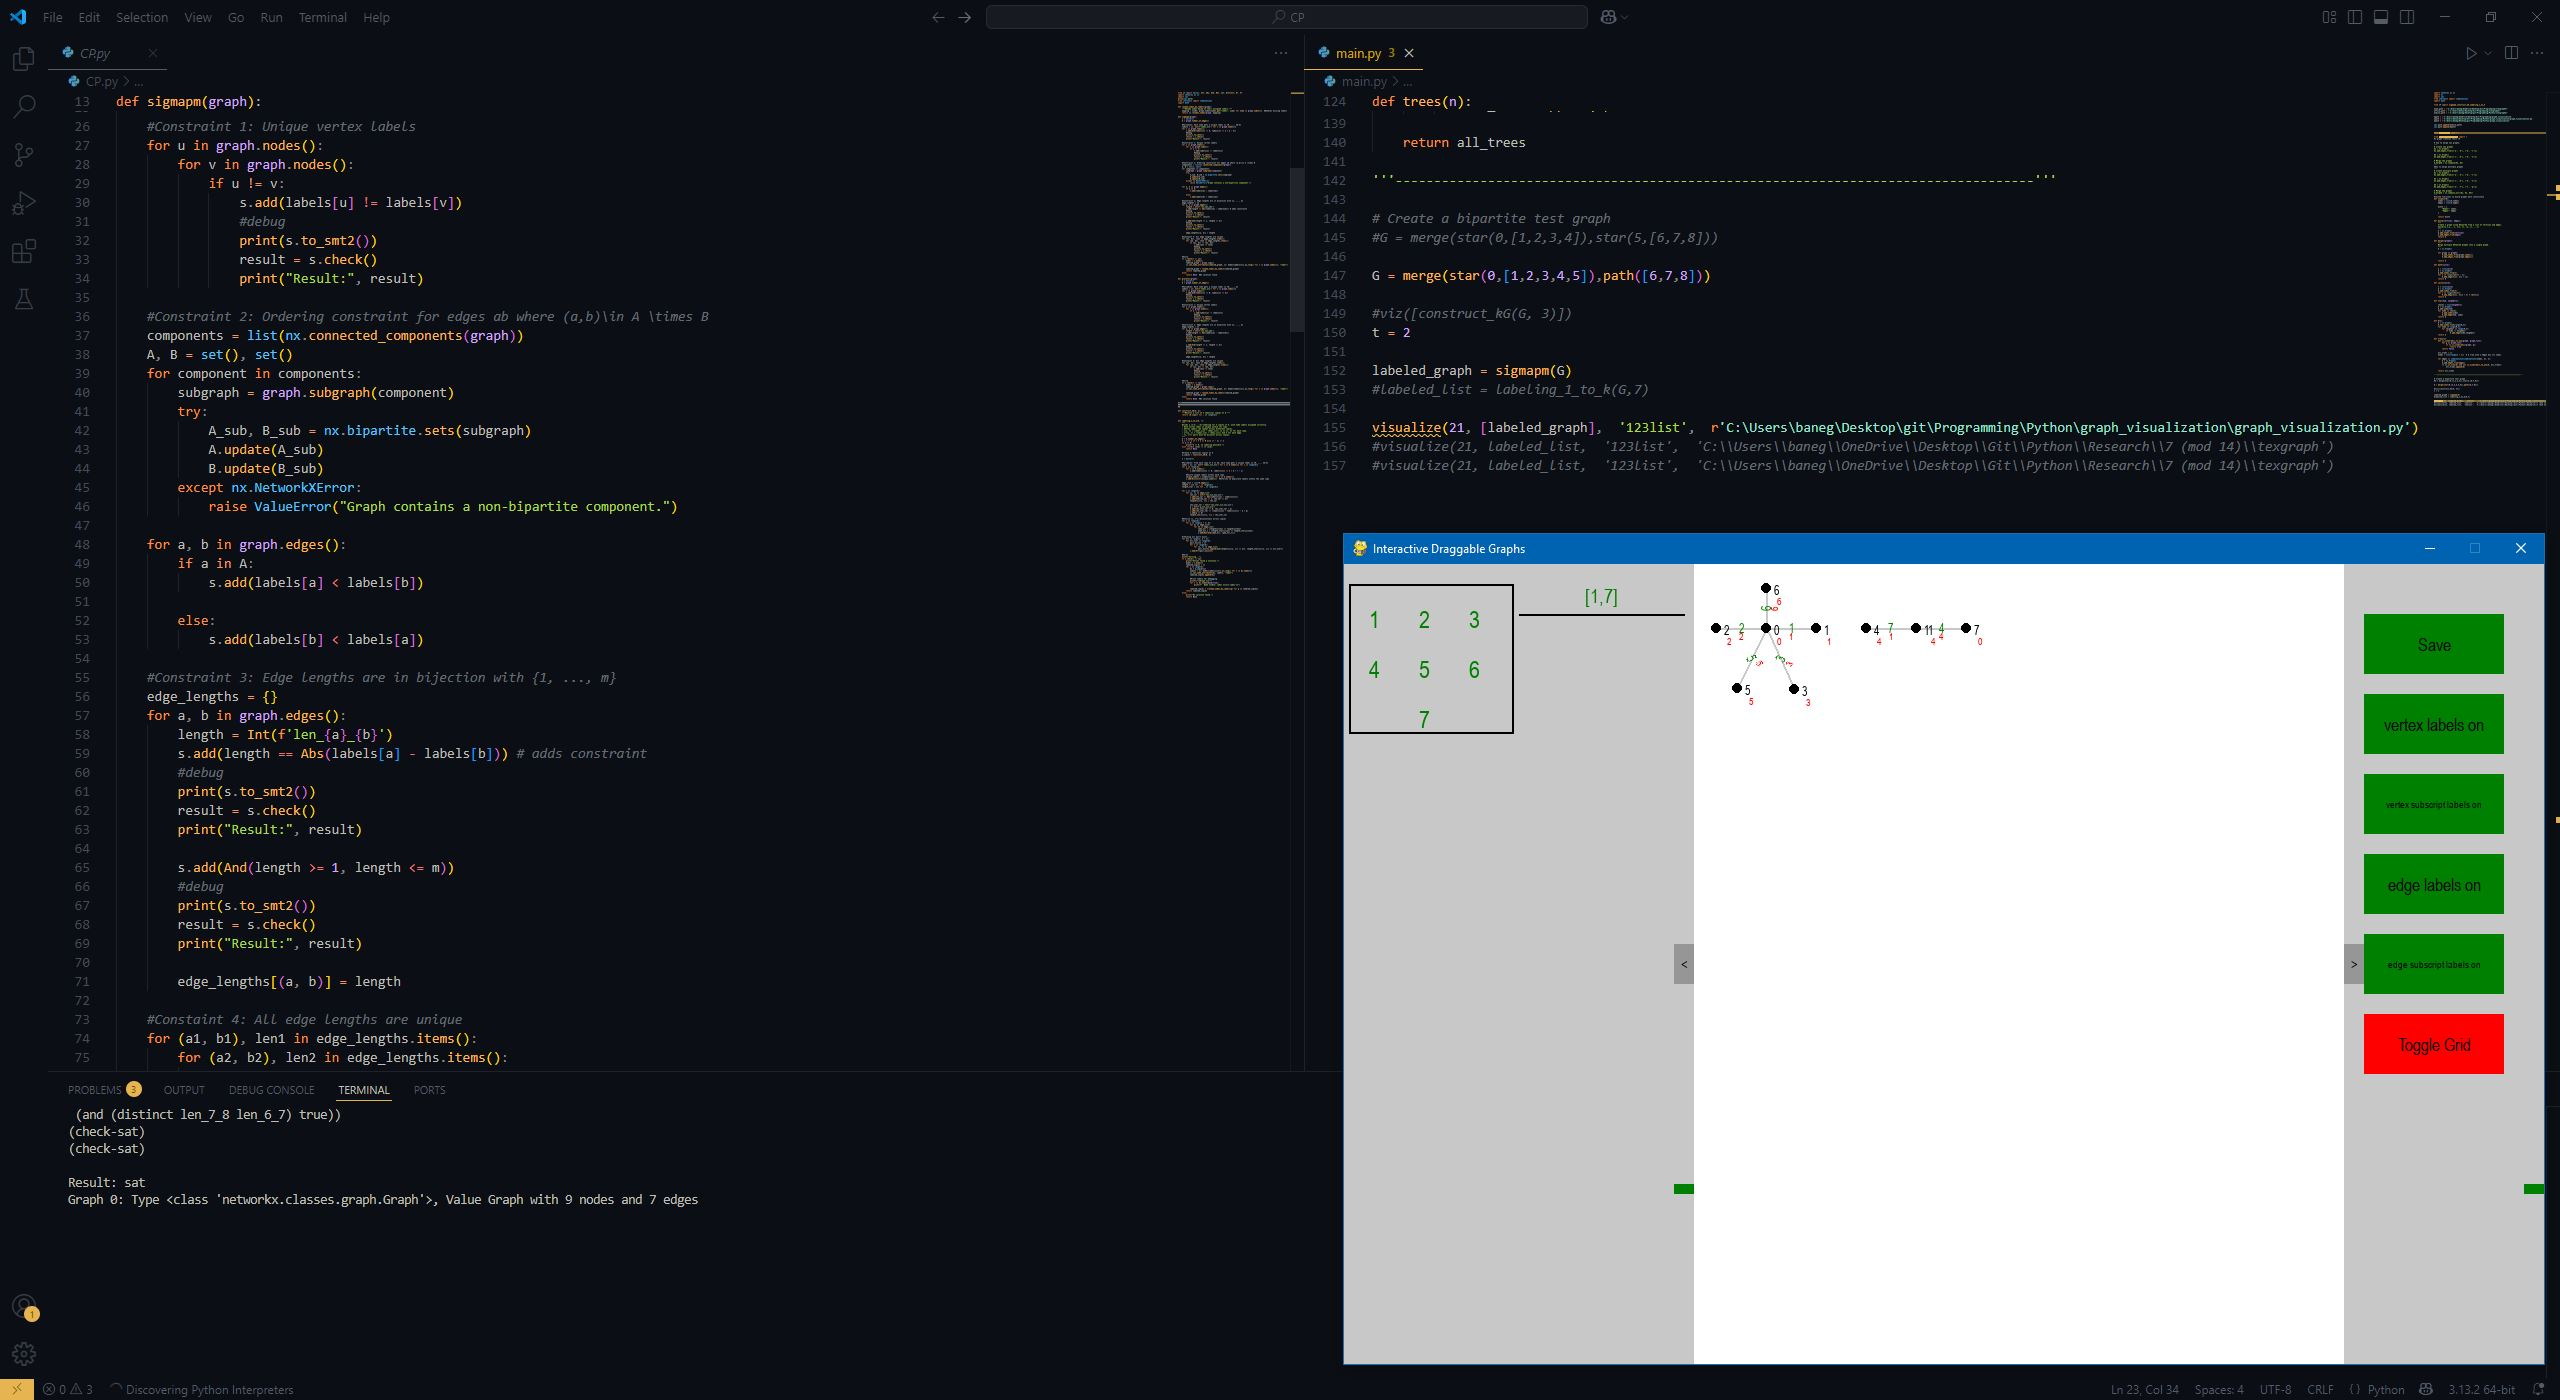
\includegraphics[width=0.8\textwidth]{standalone/Images/CPsnippetlong.JPG}
  \caption{A snippet of the $\sigma^{+-}$-labeling solver}
  \label{fig:CPsnippet}
  \end{center}
\end{figure}


These are set up so that if you visit this link: \url{https://github.com/tucxy/Thesis-Programs/tree/main} and click the code button: the .zip file installed will when extracted will give you a folder. Make that folder your working directory, and everything should just work.

\begin{figure}[H]
  \begin{center}
  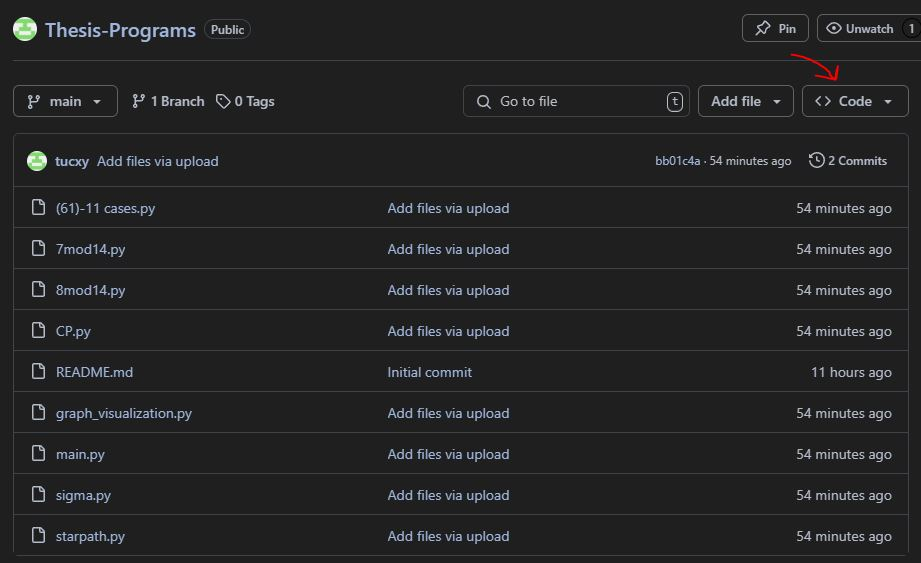
\includegraphics[width=0.8\textwidth]{standalone/Images/guide.JPG}
  \caption{click on the code button to download the zip file. Then extract the folder and set it as your working directory.}
  \label{fig:CPsnippet}
  \end{center}
\end{figure}

Feel free to email me with questions: baneg003@outlook.com